\documentclass[hidelinks,11pt]{article}
\usepackage[a4paper,width=150mm,top=30mm,bottom=35mm]{geometry}
\usepackage[utf8]{inputenc}

\usepackage{graphicx}
\graphicspath{{images/}{../images/}}

\usepackage[table]{xcolor}
\usepackage{multirow,tabularx,longtable}
\newcolumntype{Y}{>{\centering\arraybackslash}X}

%\usepackage{sectsty}
%\allsectionsfont{\nohang}

\usepackage[titletoc]{appendix}

%\usepackage{titlesec}

\usepackage[numbers]{natbib}
\renewcommand{\refname}{\large References}  % for the article class
\renewcommand{\bibname}{\large References}  % for the report or book class
\def\bibfont{\footnotesize}

% line break in bibliography urls
\usepackage{xurl}

\usepackage{caption}
%\usepackage{tocbibind}

% indent paragraphs
\usepackage{changepage}

\usepackage{mathtools}
\usepackage{amsmath}
\usepackage{amssymb}
\usepackage{amsthm}
\usepackage{color}
\usepackage{float}
\usepackage{bm}
\usepackage{multirow, makecell}
\usepackage{enumitem}
\usepackage{bold-extra}
\usepackage[mathscr]{euscript}


\usepackage{minted}
\usemintedstyle{tango}


\DeclareMathOperator{\lca}{lca}
\DeclareMathOperator*{\argmax}{arg\,max}
\DeclareMathOperator*{\argmin}{arg\,min}
\definecolor{darkgrey}{rgb}{0.2,0.2,0.2}
\newcommand{\TODO}[1]{\begingroup\color{red}#1\endgroup}
\newcommand{\OLD}[1]{\begingroup\tiny   \color{green}#1\endgroup}
\newtheorem{theorem}{Theorem}
\newtheorem{lemma}[theorem]{Lemma}
\newtheorem{corollary}[theorem]{Corollary}
\newtheorem{definition}[theorem]{Definition}
\newtheorem{fact}[theorem]{Observation}
\def\arrowedvec{\mathaccent"017E}
\newcommand{\G}{\arrowedvec{G}}
\newcommand{\unrooted}[1]{\overline{#1}}  
\newcommand{\ROOT}{\circledcirc}
\newcommand{\LEAF}{\odot}
\usepackage{wasysym}
\newcommand{\SPEC}{\newmoon}
\newcommand{\HGT}{\triangle}
\newcommand{\DUPL}{\square}
\newcommand{\child}{\mathsf{child}}
\newcommand{\degree}{\mathsf{deg}}
\newcommand{\parent}{\mathsf{par}}
\newcommand{\bmr}{\mathrel{\bm{\rightarrow}}}
\newcommand{\C}[1]{\mathscr{C}_{#1}}
\newcommand{\AX}[1]{\textnormal{#1}}

\newcommand{\COMMANDLINE}[1]{\begingroup\par\vspace{3mm}\color{darkgrey}\begin{adjustwidth}{1cm}{1cm}\texttt{#1}\end{adjustwidth}\vspace{3mm}\endgroup}


% Mark overfull boxes
\overfullrule=1mm

% Hyphenation and line breaks
\hyphenation{du-pli-ca-ti-on}

% contents links etc.
\usepackage{hyperref}
\hypersetup{
	colorlinks=True,
	linkcolor=blue,
	filecolor=magenta,      
	urlcolor=cyan,
	citecolor=black,
}

%\usepackage{setspace}

\begin{document}

\begin{titlepage}
	\begin{center}
		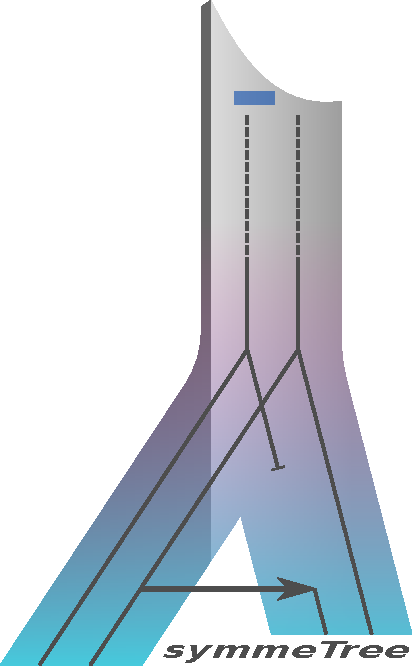
\includegraphics[width=0.4\textwidth]{logo.pdf}
	\end{center}
	\begin{center}
		\vspace*{2cm}
		
		\Huge{\fontfamily{lmtt}
			AsymmeTree User Manual
		}

		\vspace{1.5cm}
		
		\LARGE
		David Schaller\\
		\vspace{1cm}
		\large
		sdavid@bioinf.uni-leipzig.de
		
		\vspace{2cm}
		
	\end{center}
\end{titlepage}

\newpage

\tableofcontents
\newpage

\section{Introduction}

AsymmeTree is an open-source Python library for the simulation and analysis of phylogenetic scenarios.
It includes a simulator for species and gene trees with asymmetric evolution rates, tools for the inference and analysis of phylogenetic best matches \citep{geiss2019a,geiss2020c} (resp. best hits) from known gene trees or evolutionary distances. Moreover, it includes an algorithm to compute supertrees \citep{deng2016} and a method to estimate rooted species trees from an ensemble of orthology/paralogy relations \citep{hellmuth2015}.

The library, and especially the simulator, was primarily designed to be able to validate mathematical concepts and test inference methods for various steps on the way to more realistically available data, i.e., dated gene trees, additive distances of gene sets, noisy distances and finally sequences.
Both nucleotide and amino acid sequence simulation with or without indels are supported. In both cases, several substitution models are available.

The software is hosted on \href{https://github.com/david-schaller/AsymmeTree}{GitHub} and also available via The Python Package Index (\href{https://pypi.org/project/asymmetree/}{PyPI}).
Please feel free to report bugs or make suggestions for improvement in the \href{https://github.com/david-schaller/AsymmeTree/issues}{Issues} section of the GitHub repository.

If you use AsymmeTree in your project or code from it, please cite:

\vspace{3mm}
\begin{adjustwidth}{1cm}{1cm}
	Peter F. Stadler, Manuela Gei{\ss}, David Schaller, Alitzel L{\'o}pez S{\'a}nchez, Marcos Gonz{\'a}lez Laffitte, Dulce I. Valdivia, Marc Hellmuth, Maribel Hern{\'a}ndez Rosales (2020). \textbf{From pairs of most similar sequences to phylogenetic best matches.} \textit{Algorithms for Molecular Biology.} doi: 10.1186/s13015-020-00165-2. \citep{stadler2020}.
\end{adjustwidth}
\vspace{3mm}


\section{Installation}

AsymmeTree requires Python 3.5 or higher. Python 2 is not supported.

\subsection{Easy Installation with pip}


The \texttt{asymmetree} package is available on The Python Package Index (PyPI):

\COMMANDLINE{pip install asymmetree}

\noindent
For details about how to install Python packages see
\href{https://packaging.python.org/tutorials/installing-packages/}{here}.

\subsection{Installation with the setup file}


Alternatively, you can download or clone the repo, go to the root folder of package and install it using the command:

\COMMANDLINE{python setup.py install}


\subsection{Dependencies}

AssymmeTree has several dependencies (which are installed automatically when using \texttt{pip} or the \texttt{setup.py}):

\begin{itemize}
	\item \href{https://networkx.github.io}{NetworkX}
	\item \href{http://www.scipy.org/install.html}{SciPy and NumPy}
	\item \href{https://matplotlib.org/}{Matplotlib}
\end{itemize}

To use the tree reconstruction method for best match inference and the C++ implementation of the quartet method \citep{stadler2020}, the software \href{https://birc.au.dk/software/rapidnj/}{RapidNJ} \citep{simonsen2008}, resp., \href{https://github.com/david-schaller/qinfer}{qinfer} must be installed.
I recommend that you compile these tools on your machine, place the binaries into a persistent location and add this location to your PATH environment variable.
Both tools do \emph{not} need to be installed for most functionalities including the simulator.



\section{Usage}

AsymmeTree is divided into several subpackages and modules, an overview of which is given in Appendix~\ref{apx:package_structure}.
The library interface functions are described in the following sections and can be imported directly from the respective subpackage (see examples).

The term `color' regularly appears in the library and refers to the reconciliation of gene trees with species trees.
In particular, the terms `color' and `species'/`genome' in which a gene resides are used interchangeably.
The emphasizes the close connection to vertex-colored graphs such as (colored) Best Match Graphs \citep{geiss2019a}.



\subsection{Tree Data Structures}

The two classes \texttt{Tree} and \texttt{PhyloTree} (inherits from \texttt{Tree}) implement tree data structures which are essential for most of the modules in the package.
The latter contains converters and parsers for the Newick format and a NetworkX graph format.

The vertices of a \texttt{PhyloTree} instance are of type \texttt{PhyloTreeNode} and contain the following attributes:

\vspace{3mm}
\renewcommand{\arraystretch}{1.5}

{\small\centering
\begin{longtable}{ p{3.0cm} p{10cm} }
	\texttt{ID} & vertex ID (\texttt{int})\\
	\texttt{label}  & label (\texttt{str}), in gene trees: \texttt{"S"} for speciation, \texttt{"D"} for duplication, \texttt{"H"} for horizontal gene transfer, \texttt{"*"} for loss\\
	\texttt{color} & only gene trees; species in which the gene resides, i.e., ID of some vertex in a species tree, \texttt{int} for extant genes, can be of type \texttt{tuple} (of two \texttt{int}s) for inner and loss vertices\\
	\texttt{tstamp} & time stamp of the event (\texttt{double})\\
	\texttt{dist} & evolutionary distance or divergence time from the parent vertex (\texttt{double})\\
	\texttt{tranferred} & only gene trees; indicates whether the edge from the parent is the transfer edge from an HGT event; \texttt{1} if yes and \texttt{0} otherwise \\
\end{longtable}
}
\vspace{3mm}

Both species and gene trees can be converted into Newick format using the function \texttt{to\_newick()} of the \texttt{PhyloTree} class.
In case of a gene tree, the color is represented in brackets, e.g.

\begin{adjustwidth}{1cm}{1cm}\vspace{2mm}
\begin{minted}[fontsize=\footnotesize]{python}
>>> '(3<1>:0.534,2<2>:0.762)S<0>:0.273'
\end{minted}
\end{adjustwidth}

\noindent
To suppress this, use \texttt{to\_newick(color=False)}. Likewise, to suppress the distances, you can use \texttt{to\_newick(distance=False)}.
The function \texttt{PhyloTree.parse\_newick()} can handle this customized format as well as the standard Newick format.

Moreover, phylogenetic trees can easily be serialized in \texttt{json} or \texttt{pickle} (Python's serialization library) format:

\begin{adjustwidth}{1cm}{1cm}\vspace{2mm}
\begin{minted}[fontsize=\footnotesize]{python}
# tree is of type 'PhyloTree'
tree.serialize('tree.pickle')
# or
tree.serialize('tree.json')
\end{minted}
\end{adjustwidth}

\noindent
By default, the serialization format is inferred from the file extension.
Alternatively, it can be specified as keyword argument, e.g.\ \texttt{mode="json"}.
To load a tree that was serialized this way, use:

\begin{adjustwidth}{1cm}{1cm}\vspace{2mm}
\begin{minted}[fontsize=\footnotesize]{python}
from asymmetree import PhyloTree

tree = PhyloTree.load('tree.json')
\end{minted}
\end{adjustwidth}

\subsection{Simulation of Species and Gene Trees}

The subpackage \texttt{asymmetree.treeevolve} contains modules for the simulation of dated species and gene trees.
In terms of divergence time, these trees define an ultrametric on the set of their (extant) leaves.
Gene trees, furthermore, can be manipulated with a realistic rate heterogeneity among their branches resulting in general additive distances.


\subsubsection{Species Trees}

The function \texttt{simulate\_species\_tree(N)} simulates a dated species tree with \texttt{N} leaves (i.e. recent species) using the specified model.
The following models are available:

\vspace{3mm}
{\small\centering
	\begin{longtable}{ p{3.5cm} p{10cm} }
		\texttt{"innovation"} & Innovation model \citet{keller-schmidt2012}, if not specified the divergence time between the (planted) root and the leaves will be normalized to unity\\
		\texttt{"yule"}  & standard Yule model \citep{yule1924}, default birth rate is 1.0 \\
		\texttt{"BDP"} & constant-rate birth-death process \citep[see e.g.][]{kendall1948,hagen2018}, default birth rate is 1.0 and death rate is 0.0 \\
		\texttt{"EBDP"} & episodic birth-death process, algorithm of \cite{stadler2011} \\
	\end{longtable}
}
\vspace{3mm}

\noindent
The following keyword parameters (with their default value) are available:

\vspace{3mm}
{\small\centering
\begin{longtable}{ p{3.5cm} p{10cm} }
	\texttt{model="innovation"}  & model for the species tree simulation, currently only the `innovation model' is available\\
	\texttt{non\_binary\_prop=0.0} & probability that an inner edge is contracted,
	results in a non-binary tree\\
	\texttt{planted=True} & add a planted root that has the first true speciation node as its
	single neighbor, this way duplication (and loss) events can occur before the first speciation event in a subsequent gene tree simulation\\
	\texttt{remove\_extinct=\newline False} & remove all branches leading to losses, only relevant for models with death events\\
	\texttt{rescale\_to\_height=\newline None} & specify the divergence time between the (planted) root and the leaves i.e.\ the final height of the dated tree\\
\end{longtable}
}
\vspace{3mm}

For any model, the root of the resulting tree has the maximal time stamp and all (extant) species have time stamp 0.0.
The episodes of the \texttt{"EBDP"} model must be supplied as a list of tuples/lists where each episode has the structure

\begin{adjustwidth}{1cm}{1cm}\vspace{2mm}
\begin{minted}[fontsize=\footnotesize]{python}
(birthrate, deathrate, proportion_of_survivors, time_stamp).
\end{minted}
\end{adjustwidth}

\noindent
Note that the first elements in this list correspond to the most recent ones, and that the first episode should have a time stamp of 0.0.
Example usage:

\begin{adjustwidth}{1cm}{1cm}\vspace{2mm}
\begin{minted}[fontsize=\footnotesize]{python}
import asymmetree.treeevolve as te

S1 = te.simulate_species_tree(10, planted=True, non_binary_prob=0.2)
print(S1.to_newick())

S1 = te.simulate_species_tree(10, model='EBDP',
                              episodes=[(1.0, 0.3, 0.8, 0.0),
                                        (0.9, 0.4, 0.6, 0.3)])
print(S2.to_newick())
\end{minted}
\end{adjustwidth}


\subsubsection{Gene Trees}

Dated gene trees are simulated along a given species tree \texttt{S} with a variant of the birth-death, resp., Gillespie algorithm \citep{kendall1948,gillespie1976}.
To this end, use the class \texttt{GeneTreeSimulator} or the function \texttt{simulate\_dated\_gene\_tree(S, **kwargs)} with a species tree of type \texttt{PhyloTree}.
The following parameters are available:

\vspace{3mm}
{\small\centering
\begin{longtable}{ p{4.0cm} p{9cm} }
	\texttt{DLH\_rates=\newline (0.0, 0.0, 0.0)} & a \texttt{tuple} of three \texttt{float}s, rates for duplication, loss and horizontal gene transfer (HGT) events\\
	\texttt{dupl\_polytomy=0.0}  & allows non-binary duplication events by specifying
	the parameter~$\lambda$ of a Poisson distribution (copy number = 2 + drawn number)\\
	\texttt{prohibit\_extinction=\newline "per\_species"}  & avoid loss events for genes that are the last survivor in their species branch (\texttt{"per\_species"}), the last survivor of the whole family (\texttt{"per\_family"}); or no constraints  (\texttt{False})
\end{longtable}
}
\vspace{3mm}

\noindent
For the constraints to avoid extinction, the loss rate in the respective branches are temporarily set to zero.
Example usage:

\begin{adjustwidth}{1cm}{1cm}\vspace{2mm}
\begin{minted}[fontsize=\footnotesize]{python}
import asymmetree.treeevolve as te

# S is a species tree of type PhyloTree
tree_simulator = te.GeneTreeSimulator(S)
tree = tree_simulator.simulate(DLH_rates=(1.0, 0.5, 0.1))

# or
tree = te.simulate_dated_gene_tree(S, DLH_rates=(1.0, 0.5, 0.1))
\end{minted}
\end{adjustwidth}

The function \texttt{observable\_tree(tree)} returns the observable part of a gene tree, i.e., it copies the tree, removes all branches that lead to loss events only and suppresses all inner nodes with only one child. 
It also removes the planted root.
Example usage:
\begin{adjustwidth}{1cm}{1cm}\vspace{2mm}
\begin{minted}[fontsize=\footnotesize]{python}
# observable gene tree
ogt = ts.observable_tree(tree)
\end{minted}
\end{adjustwidth}


\subsubsection{Assignment of Variable Evolution Rates}

The module \texttt{EvolutionRates} contains functions to model realistic (asymmetric) evolution rates for a given gene tree.
Moreover, correlation of the evolution rates between genes of the same (and closely related) species is introduced (autocorrelation, \citep{kishino2001}).
The function \texttt{assign\_rates(T, S)} takes a gene tree \texttt{T} and the \textbf{corresponding} species tree \texttt{S} as input, and manipulates the branch length of the gene tree.
The following keyword parameters (with their default values) are available:

\vspace{3mm}
{\small\centering
\begin{longtable}{ p{4.0cm} p{9cm} }
	\texttt{base\_rate=1.0} & starting value for the substitution rate (per time unit) and expected value for conserved genes\\
	\texttt{autocorr\_factors=None}  & a dictionary containing rate factors for the edges of the species tree\\
	\texttt{autocorr\_variance=0.0}  & variance factor for a lognormal distribution that controls autocorrelation between genes of the same (and closely related) species, the higher the lower the auto\-corre\-la\-tion; only relevant if \texttt{autocorr\_factors} is not directly supplied\\
	\texttt{gamma\_param=\newline (0.5, 1.0, 2.2)}  & parameter the for Gamma distribution (\texttt{a, loc, scale}) from which rate factors for divergent are drawn, the default values are chosen to fit observed asymmetries between paralogs in yeast data \citep{byrne2007}\\
	\texttt{CSN\_weights=(1, 1, 1)}  & weights for choice between conservation,
	subfunctionalization and neofunctionalization after a duplication event\\
	\texttt{inplace=True}  & manipulate edge lengths (\texttt{dist}) of the gene tree in-place, otherwise copy the tree\\
\end{longtable}
}
\vspace{3mm}

\noindent
It is recommended to apply the rate assignment to the true gene tree that still contains loss events.
Note that the rates are used to manipulate the \texttt{dist} attributes in the gene tree and not returned explicitly.
Example usage:
\begin{adjustwidth}{1cm}{1cm}\vspace{2mm}
\begin{minted}[fontsize=\footnotesize]{python}
import asymmetree.treeevolve as te

S = te.simulate_species_tree(10)

# true gene tree (with losses)
tree = te.simulate_dated_gene_tree(S, DLH_rates=(0.5, 0.5, 0.5))
te.assign_rates(tree, S, base_rate=1,
                autocorr_variance=0.2,
                gamma_param=(0.5, 1.0, 2.2))
                
# or in a single step
tree = simulate_gene_trees(S, N=1,
                           DLH_rates=(0.5, 0.5, 0.5)
                           base_rate_distr=('constant', 1.0),
                           autocorr_variance=0.2,
                           gamma_param=(0.5, 1.0, 2.2))

# observable gene tree
ogt = ts.observable_tree(tree)
\end{minted}
\end{adjustwidth}

\noindent
The function \texttt{simulate\_gene\_trees(S)} combines the simulation of dated gene trees and the rate assignment into one step.
If \texttt{N=1}, a single gene tree is returned.
Otherwise, a list of gene trees is returned that shared the same rate factors for the branches in the species tree (autocorrelation factors) in the rate assignment procedure.
Moreover, a distribution for the base rate (assigned the planted edge of the gene tree) can be specified with the parameter \texttt{base\_rate\_distr}.
Available are e.g.\ \texttt{("constant", rate)} and \texttt{("gamma", shape, scale)}.


\subsubsection{Distance Matrix and Noise}

Distances derived from (real-life) gene or protein sequences are always burdened with noise.
Such data can either be modeled by simulating sequences, or by disturbing the distances specified by a given tree directly.
The latter alternatively is described briefly in this section.

The additive (i.e.\ noiseless) distance from an \textbf{observable} gene tree can be computed using the function \texttt{distance\_matrix()} of a \texttt{PhyloTree} instance.
It returns a tuple containing a list of leaves in the tree (corresponding to the row/column order) and the distance matrix as a 2-dimensional \texttt{numpy} array.

\begin{adjustwidth}{1cm}{1cm}\vspace{2mm}
\begin{minted}[fontsize=\footnotesize]{python}
# tree is an observable gene tree
leaves, D = tree.distance_matrix()
leaf_index_dict = {leaf: i for i, leaf in leaves}
\end{minted}
\end{adjustwidth}

In the next step, noise can be introduced into a distance matrix using the \texttt{NoisyMatrix} module.
Random noise can be simulated with the function \texttt{noisy\_matrix(orig\_matrix, sd)}.
The following parameters are available (keyword arguments are indicated by their default value):

\vspace{3mm}
{\small\centering
\begin{longtable}{ p{4.5cm} p{9cm} }
	\texttt{orig\_matrix} & original matrix to be disturbed\\
	\texttt{sd}  & standard deviation of a normal distribution with mean 1 from which noise factors are drawn\\
	\texttt{metric\_repair="reject"}  & method to ensure that the resulting distance matrix is still a metric, available are the rejection of noise steps that violate the metric property (\texttt{"reject"}), the decrease-only metric repair (\texttt{"DOMR"}) and the general metric repair (\texttt{"general"}) algorithm\\
\end{longtable}
}
\vspace{3mm}

Alternatively, the function \texttt{convex\_linear\_comb(D1, D2)} can be used to simulate systematically biased noise by computing a linear convex combination with a disturbance matrix.
The function thus takes two distance matrices (\texttt{numpy} arrays) not necessarily of the same size as input and disturbs them with one another.
The contribution of the respective disturbance matrix is controlled by the keyword parameter \texttt{alpha} (default is \texttt{0.5}).
If the keyword parameter \texttt{first\_only} is specified as \texttt{True}, only the first disturbed matrix is returned.
Otherwise, both are returned in a tuple.


\subsection{Simulation of Sequences}

AsymmeTree supports the simulation of nucleic and amino acid sequences using time-continuous Markov models, as usually applied for this purpose \citep[for textbooks, see e.g.][]{felsenstein2004,yang2006,yang2014}.
The subpackage \texttt{asymmetree.seqevolve} contains the modules and functions for this task.

The class \texttt{Evolver} takes several model as parameters for its initialization:
\begin{itemize}
	\item a \textbf{subtitution} model (\texttt{SubstModel}, required) for the substitution of single bases or amino acids,
	\item an \textbf{indel} model (\texttt{IndelModel}, optional) for the simulation of insertions and/or deletion, and
	\item a model for rate \textbf{heterogeneity} (\texttt{HetModel}, optional) among the sites of the sequence under evolution 
\end{itemize}

\subsubsection{Substitution Model}

A substitution model usually comprises an exchangeability matrix $S$ and a vector $\pi$ containing the equilibrium frequencies of the alphabet $A$ of nucleobases, amino acids et cetera.
From this, the rate matrix $Q$ can be computed as $S\Pi$ where $\Pi=\textrm{diag}\{\pi_1,\dots,\pi_{|A|}\}$ \citep{yang2006}.
The substitution probability matrix, in turn, is given by \[P=e^{Qt}\] which is computed efficiently by AsymmeTree using matrix diagonalization.

The following models for nucleotide (\texttt{n}) and amino acid (\texttt{a}) substitution are currently available (codon models are not supported at the moment):

\vspace{3mm}
{\small\centering
	\begin{longtable}{ p{1.5cm} p{1.0cm} p{5.5cm} p{5.5cm}}
		% ---------------------------------------------------
		model & type & reference & required parameters (\texttt{kwargs})\\
		% ---------------------------------------------------
		\texttt{JC96} & \texttt{n}/\texttt{a} & Jukes \& Cantor 1969 \citep{jukes1969} & \texttt{-}\\
		% ---------------------------------------------------
		\texttt{K80} & \texttt{n} & Kimura 1980 \citep{kimura1980} & \texttt{kappa} (transition/transversion rate ratio)\\
		% ---------------------------------------------------
		\texttt{GTR} & \texttt{n} & general time-reversable model (GTR) 1986 \citep{tavare1986} & \texttt{abcdef} (list of rates (a) $C\leftrightarrow T$, (b) $A\leftrightarrow T$, (c) $G\leftrightarrow T$, (d) $A\leftrightarrow C$, (e) $C\leftrightarrow G$, (f) $A\leftrightarrow G$);\newline
		\texttt{f} (list of equilibrium frequencies $A/C/G/T$)\\
		% ---------------------------------------------------
		\texttt{DAYHOFF} & \texttt{a} & Dayhoff 1978 \citep{dayhoff1978} & \texttt{-}\\
		% ---------------------------------------------------
		\texttt{BLOSUM62} & \texttt{a} & BLOSUM62 1992 \citep{henikoff1992} & \texttt{-}\\
		% ---------------------------------------------------
		\texttt{JTT} & \texttt{a} & Jones, Taylor \& Thornton 1992 \citep{jones1992} & \texttt{-}\\
		% ---------------------------------------------------
		\texttt{WAG} & \texttt{a} & Whelan \& Goldman 2001 \citep{whelan2001} & \texttt{-}\\
		% ---------------------------------------------------
		\texttt{LG} & \texttt{a} & Le \& Gascuel 2008 \citep{le2008} & \texttt{-}\\
		% ---------------------------------------------------
		\texttt{CUSTOM} & \texttt{n}/\texttt{a} & \texttt{-} & \texttt{filename} (path to a file with a model in PAML \citep{yang1997} format)\\
		% ---------------------------------------------------
	\end{longtable}
}
\vspace{3mm}

Note that a custom substitution model can be specified via \texttt{model\_name="CUSTOM"}.
In this case, the path to the model in PAML \citep{yang1997} format must be supplied.
Moreover, the model type (\texttt{n}/\texttt{a}) must fit this model.
Example usage:

\begin{adjustwidth}{1cm}{1cm}\vspace{2mm}
\begin{minted}[fontsize=\footnotesize]{python}
from asymmetree.seqevolve import SubstModel

# non-empirical model
subst_model_jc69 = SubstModel('n', 'K80', kappa=2.0)

# empirical model
subst_model_jtt = SubstModel('a', 'JTT')

# custom model
subst_model_custom = SubstModel('a', 'CUSTOM', filename='path/to/custom.paml')
\end{minted}
\end{adjustwidth}


\subsubsection{Indel Model}

Insertions and deletions are modeled based on \texttt{Dawg} \citep{cartwright2005}.
An indel model requires sitewise rates for insertion \texttt{insertion\_rate} and deletion \texttt{deletion\_rate}.
Moreover, the following parameters are available (with default values):

\vspace{3mm}
{\small\centering
\begin{longtable}{ p{4.5cm} p{9cm} }
	\texttt{length\_model="zipf"} & distribution of indel length\\
	\texttt{max\_length=False} & integer max.\ value at which the specified distribution is truncated, must be greater than the expected value of the distribution, \texttt{False} means no limit\\
\end{longtable}
}
\vspace{3mm}

\noindent
The following models for indel length are available:

\vspace{3mm}
{\small\centering
\begin{longtable}{ p{3.5cm} p{3.5cm} p{5cm}}
	% ---------------------------------------------------
	model & distribution & required parameters (\texttt{kwargs}, with default values)\\
	% ---------------------------------------------------
	\texttt{zipf} & Zipf & \texttt{a=1.821} \citep{chang2004} (parameter $a$ of the Zipf distribution)\\
	% ---------------------------------------------------
	\texttt{negative\_binomial} & negative binomial & \texttt{r=1.0} and \texttt{q=0.5} (parameters $r$ and $q$ of the negative binomial distribution)\\
	% ---------------------------------------------------
\end{longtable}
}
\vspace{3mm}

\noindent
Example usage:

\begin{adjustwidth}{1cm}{1cm}\vspace{2mm}
\begin{minted}[fontsize=\footnotesize]{python}
from asymmetree.seqevolve import IndelModel

# sitewise insertion rate 0.01 and deletion rate 0.008
indel_model = IndelModel(0.01, 0.008, length_model='zipf', a=2.0)
\end{minted}
\end{adjustwidth}


\subsubsection{Heterogeneity Model}

Selective pressure usually varies among the sites of a sequence under evolution.
To model this, rate factors $r$ for single sites or groups of sites are commonly drawn from a Gamma distribution (`$+\Gamma$') with mean 1 and parameter $\alpha$ \citep{cartwright2005,fletcher2009,dalquen2012}.
The rate matrix $rQ$ is then used instead of $Q$.
Note that smaller values for $\alpha$ correspond to higher heterogeneity.

AsymmeTree supports two modes of the `$+\Gamma$'-model.
You can specify a number of classes to which the sites are assigned randomly and uniformly distributed.
Sites of the same class share a common factor $r$.
The other possibility is a sitewise heterogeneity, i.e., every site has its own rate.
In both cases, the rate or class membership is inherited from the parent sites during the evolution along a tree.
Note that the sitewise mode is expected to have a longer running time.

An other aspect of among site heterogeneity is the modeling of invariant sites (`$+I$'), i.e., sites that never mutate at all as a result of very strong selective pressure.
The (expected) proportion $p$ of invariant sites can be specified by the user, and sites are assigned as \texttt{"invariant"} with probability $p$.
Note that $p>0$ affects the overall substitution rate.
In other words, the rates of the non-invariant sites are \textbf{not} adjusted to compensate the decreased number of expected substitution over all sites.

To summarize, the following parameters are available for the class \texttt{HetModel} (keyword arguments are indicated by their default value):

\vspace{3mm}
{\small\centering
\begin{longtable}{ p{4.5cm} p{9cm} }
	\texttt{alpha} & parameter $\alpha$ of the Gamma distribution\\
	\texttt{classes=5} & number of classes; sites in the same class share the same rate factor\\
	\texttt{sitewise=False} & if \texttt{True}, factors are drawn sitewise; the number of classes is ignored in this case\\
	\texttt{invariant=0.0} & (expected) proportion $p$ of invariant sites\\
\end{longtable}
}
\vspace{3mm}

Note that the `$+I$'-model can be used without the `$+\Gamma$'-model by setting \texttt{classes=1} (the single class will have a factor of 1) and \texttt{invariant} to some proportion greater than~0.
Example usage:

\begin{adjustwidth}{1cm}{1cm}\vspace{2mm}
\begin{minted}[fontsize=\footnotesize]{python}
from asymmetree.seqevolve import HetModel

# +G
het_model_g  = HetModel(1.5, classes=10)

# +G +I
het_model_gi = HetModel(2.0, sitewise=True, invariant=0.2)

# +I (value of alpha is irrelevant)
het_model_i  = HetModel(1.0, classes=1, invariant=0.25)
\end{minted}
\end{adjustwidth}


\subsubsection{The Class \texttt{Evolver}}

The class \texttt{Evolver} evolves a sequence according to the specified models (see previous sections) along a phylogenetic tree.
In AsymmeTree, the \textbf{\texttt{dist}} attribute of the vertex $v$ in an edge $uv$ of the tree ($u$ is closer to the root) is always used as the \textbf{expected number of substitutions} along this edge.
Thus, PAM distances as e.g.\ used optionally in \citep{dalquen2012} are not supported.
The \texttt{dist} attribute is also used as the duration of the Markov process in which insertions and deletions are drawn.

The following parameters are available for the initialization of an \texttt{Evolver} instance (keyword arguments are indicated by their default value):

\vspace{3mm}
{\small\centering
	\begin{longtable}{ p{4.5cm} p{9cm} }
		\texttt{subst\_model} & substitution model; instance of \texttt{SubstModel}\\
		\texttt{indel\_model=None} & model for insertions and deletions; instance of \texttt{IndelModel}\\
		\texttt{het\_model=None} & model for among site heterogeneity and invariant sites; instance of \texttt{HetModel}\\
		\texttt{jump\_chain=False} & if \texttt{True}, an alternative Gillespie-like \citep{gillespie1976} algorithm is applied for the substitution process instead of the computation of $P=e^{Qt}$ \\
	\end{longtable}
}
\vspace{3mm}

Once the \texttt{Evolver} is initialized, its function \texttt{evolve\_along\_tree()} can be called to evolve a sequence along a tree.
The following parameters are available for this function (keyword arguments are indicated by their default value):

\vspace{3mm}
{\small\centering
	\begin{longtable}{ p{4.5cm} p{9cm} }
		\texttt{tree} & phylogenetic tree; instance of \texttt{PhyloTree}\\
		\texttt{start\_length=200} & length of the root sequence which is randomly drawn from the equilibrium frequencies in the specified substitution model\\
		\texttt{start\_seq=None} & root sequence (\texttt{str}); must be compatible with the specified substitution model (\texttt{model\_type="n"/"a"}); if supplied, the \texttt{start\_length} attribute is ignored\\
	\end{longtable}
}
\vspace{3mm}

\noindent
The sequences of a simulation run are returned by this function (and also available via the attribute \texttt{sequences} as long as the function has not been called again), which is a \texttt{dict} containing the nodes (inner and leaf nodes) as keys and instances of type \texttt{EvoSeq} as values.
The latter can be converted into \texttt{str} using \texttt{subst\_model.to\_sequence(evo\_seq)}.

The function \texttt{true\_alignment()} can be used to compute (and optionally write into a file) the `true' alignment of a simulation run.
The following keyword parameters are available:

\vspace{3mm}
{\small\centering
	\begin{longtable}{ p{4.5cm} p{9cm} }
		\texttt{include\_inner=True} & if \texttt{True}, include also inner nodes in the alignment; otherwise only sequences of leaf nodes are aligned\\
		\texttt{write\_to=None} & path and filename for the output\\
		\texttt{alignment\_format=\newline "phylip"} & format of the alignment file; available are \texttt{"phylip"}, \texttt{"clustal"} and \texttt{"pretty"}\\
	\end{longtable}
}
\vspace{3mm}

Example usage of the class \texttt{Evolver}:

\begin{adjustwidth}{1cm}{1cm}\vspace{2mm}
\begin{minted}[fontsize=\footnotesize]{python}
from asymmetree.seqevolve import Evolver, SubstModel, IndelModel, HetModel

# specify models (only 'SubstModel' is mandatory)
subst_model = SubstModel('a', 'WAG')
indel_model = IndelModel(0.01, 0.01, length_model='zipf')
het_model  = HetModel(2.0, classes=7, invariant=0.1)

# evolve sequences along a phylogenetic tree 'tree'
evolver = Evolver(subst_model, indel_model=indel_model, het_model=het_model)
evolver.evolve_along_tree(tree, start_length=150)

# print resulting sequences
for node, evo_seq in evolver.sequences.items():
    print(node.label, subst_model.to_sequence(evo_seq))

# output true alignment
evolver.true_alignment(write_to='path/to/alignment.phylip',
                       alignment_format='phylip')
\end{minted}
\end{adjustwidth}


\subsection{Simulation of Genomes}


\subsection{Best Match Inference}

Phylogenetic best matches of a gene $x$ of species $X$ are defined as those genes $y$ of another species $Y\ne X$ that share the lowest common ancestor with $x$ in the gene tree among all genes in that species \citep{geiss2019a,geiss2020b,geiss2020c}.
In contrast, two genes are orthologs if their last common ancestor was a speciation event.
Orthology and reciprocal best matches are closely related~\citep{geiss2020c}.

The subpackage \texttt{asymmetree.best\_matches} contains functions to compute both relations from a given gene tree or to estimate them from distance data on a set of genes~\citep{stadler2020}.
If the true (observable) gene tree is known (as e.g.\ the case in simulations), best matches and orthologs can be computed using the module \texttt{TrueBMG}.
The functions \texttt{BMG\_from\_tree()} and \texttt{orthology\_from\_tree()} return the respective graph representation as NetworkX (Di)Graphs:

\begin{adjustwidth}{1cm}{1cm}\vspace{2mm}
\begin{minted}[fontsize=\footnotesize]{python}
from asymmetree.best_matches import orthology_from_tree, BMG_from_tree

# tree is an observable gene tree
orthology_graph = orthology_from_tree(tree)

# Best Match Graph and Reciprocal Best Match Graph as a tuple
bmg, rbmg = BMG_from_tree(tree, supply_RBMG=True)
\end{minted}
\end{adjustwidth}

\noindent
If only distance data is available, best matches have to be estimated.
AsymmeTree currently implements three different methods that are described by \citet{stadler2020}:
\begin{itemize}
	\item Extended Best Hits (module \texttt{ExtBestHits})
	\item Neighborjoining \cite{saitou1987} and midpoint rooting (module \texttt{TreeReconstruction}, requires the installation and accessibility of \texttt{RapidNJ} \citep{simonsen2008})
	\item Quartet method (module \texttt{Quartets}, Python implementation and wrapper for the C++ tool \texttt{qinfer})
\end{itemize}

Please see the file \texttt{examples/best\_match\_infer.py} in the GitHub repo for an example usage of these modules following the simulation of gene tree scenarios.



\subsection{Supertree Computation}

The module \texttt{BuildST} contains an implementation of the BuildST algorithm described by \citet{deng2016} to compute a supertree from a given list of tree based on the leaf labels.
The algorithm uses the dynamic graph data structure described by \citet{henzinger1995} and \citet{holm2001}.
The latter can also be used separately:

\begin{adjustwidth}{1cm}{1cm}\vspace{2mm}
\begin{minted}[fontsize=\footnotesize]{python}
from asymmetree.tools import HDTGraph
\end{minted}
\end{adjustwidth}

The class \texttt{BuildST} is initialized with a list of trees that are of type \texttt{Tree} (thus also \texttt{PhyloTree} is allowed).
The method \texttt{run()} then returns a supertree if the trees in the list are compatible \emph{and} they overlap in their sets of leaf labels.
More precisely, the graph on the set of input trees, in which two trees are connected by an edge if and only if they have at least one leaf label in common, must be connected.
Example usage:

\begin{adjustwidth}{1cm}{1cm}\vspace{2mm}
\begin{minted}[fontsize=\footnotesize]{python}
from asymmetree.tools import BuildST

# tree_list is a list of 'Tree' instances
st_builder = BuildST(tree_list)
supertree = st_builder.run()

if supertree:
    print(supertree.to_newick())
else:
    print('could not build a supertree')
\end{minted}
\end{adjustwidth}



\subsection{Cograph Editing and ParaPhylo}

The subpackages \texttt{asymmetree.cograph} and \texttt{asymmetree.proteinortho} contain heuristics for cograph editing and a method to compute rooted species tree from orthology/paralogy relations.
The latter is a reimplementation of \href{http://pacosy.informatik.uni-leipzig.de/208-0-ParaPhylo.html}{ParaPhylo} \citep{hellmuth2015} which uses heuristics for the NP-hard steps instead of exact ILP solutions.
For cograph editing, the $\mathcal{O}(n^2)$ algorithm (where $n$ is the number of vertices in a connected graph) by \citet{crespelle2019} is applied.
For the Maximum Consistent Triple Set problem, tree different heuristics are available:
\begin{itemize}
	\item \texttt{BPMF}: Best-Pair-Merge-First \citep{wu2004} (modified for weighted triples)
	\item \texttt{MINCUT}: Aho's \texttt{BUILD} with weighted MinCut \citep{aho1981,byrka2010}
	\item \texttt{GREEDY}: a greedy approch based on Aho's \texttt{BUILD}
\end{itemize}

The class \texttt{TreeReconstructor} in the module \texttt{SpeciesTreeFromParalogs} computes a species tree after it is provides with one or more NetworkX graphs that represent (estimated) orthology relations.
To this end, the nodes in these graph must have a \texttt{"color"} attribute, since these will be the leaf labels in the reconstructed species tree.
Example usage:

\begin{adjustwidth}{1cm}{1cm}\vspace{2mm}
\begin{minted}[fontsize=\footnotesize]{python}
from asymmetree.paraphylo import TreeReconstructor

tree_reconstr = TreeReconstructor()

# ortho_relations is a list of orthology relations
for graph in ortho_relations:
    tree_reconstr.add_ortho_graph(graph)
    
# finally an estimate the species tree can be computed
tree = tr.build_species_tree(mode='BPMF')
print(tree.to_newick())
\end{minted}
\end{adjustwidth}

The module \texttt{SpeciesTreeFromProteinOrtho} contains functions to estimate a species tree from a \texttt{ProteinOrtho} \citep{lechner2011} output file. For example, the function \texttt{reconstruct\_from\_ proteinortho(filename, triple\_mode="BPMF")} takes the filename to the output file and optionally the triple heuristic as input, and returns a tuple consisting of the estimated species tree (\texttt{PhyloTree}) and a Newick representation (\texttt{str}) containing support values for the inner nodes.

\bibliographystyle{plainnatnourl}
\bibliography{AsymmeTree}

\newpage


\appendix

\section{Subpackages and Modules}\label{apx:package_structure}

{\footnotesize
\setlength{\tabcolsep}{6pt}
\renewcommand{\arraystretch}{1.4}
%\renewcommand\tabularxcolumn[1]{m{#1}}
\begin{longtable}{| p{4.0cm} | p{10cm} |}
	\endfirsthead
	\multicolumn{2}{c}{\textit{Table continued from previous page}}\\
	\hline
	\endhead
	\hline \multicolumn{2}{r}{\textit{Table continued on next page}} \\
	\endfoot
	\hline
	\endlastfoot
	%
	\hline
	%--------------------------------------------------------------------------
	\textbf{Packages and Modules} & \textbf{Description} \\
	%--------------------------------------------------------------------------
	\hline
	%--------------------------------------------------------------------------
	\multicolumn{2}{|l|}{\textbf{\texttt{treeevolve}}}\\
	%--------------------------------------------------------------------------
	\hline
	%--------------------------------------------------------------------------
	\texttt{SpeciesTree} & 
	Simulator for dated species trees with different models. \\
	%--------------------------------------------------------------------------
	\texttt{GeneTree} & 
	Simulator for dated gene trees, construction of the observable gene tree. \\
	%--------------------------------------------------------------------------
	\texttt{EvolutionRates} & 
	Simulation of evolution rate asymmetries, autocorrelation between ancestors and descendants as well as correlation between genes in the same species. \\
	%--------------------------------------------------------------------------
	\texttt{Scenario} & 
	Wrapper class for species and gene tree scenarios, computation of the (R)BMG as well as event counts and some statistics. \\
	%--------------------------------------------------------------------------
	\texttt{NoisyMatrix} & 
	Generation of a noisy matrix (random perturbation or wrong topology noise). \\
	%--------------------------------------------------------------------------
	\hline
	%--------------------------------------------------------------------------
	\multicolumn{2}{|l|}{\textbf{\texttt{seqevolve}}}\\
	%--------------------------------------------------------------------------
	\hline
	%--------------------------------------------------------------------------
	\texttt{Evolver} & 
	Includes the class \texttt{Evolver} for the simulation of sequences along a phylogenetic tree. \\
	%--------------------------------------------------------------------------
	\texttt{EvolvingSequence} & 
	Data structure for sequences that are under evolution based on a doubly-linked list. \\
	%--------------------------------------------------------------------------
	\texttt{SubstModel} & 
	Substitution model for the sequence simulation. \\
	%--------------------------------------------------------------------------
	\texttt{IndelModel} & 
	Insertion/deletion (indel) model. \\
	%--------------------------------------------------------------------------
	\texttt{HetModel} & 
	Model for rate heterogeneity among the sites of an evolving sequence and for invariant sites. \\
	%--------------------------------------------------------------------------
	\texttt{Alignment} & 
	Construction of the true multiple sequence alignment after the simulation of sequences along a tree. \\
	%--------------------------------------------------------------------------
	\texttt{EmpiricalModels} & 
	Contains rate matrices and equilibrium frequencies for the empirical substitution models, taken from \citep{criscuolo}. \\
	%--------------------------------------------------------------------------
	\hline
	%--------------------------------------------------------------------------
	\multicolumn{2}{|l|}{\textbf{\texttt{tools}}}\\
	%--------------------------------------------------------------------------
	\hline
	%--------------------------------------------------------------------------
	\texttt{Tree} & 
	Includes the basic class \texttt{Tree}, provides functions for tree traversals, Newick parser, etc. \\
	%--------------------------------------------------------------------------
	\texttt{PhyloTree} & 
	Includes the class \texttt{PhyloTree} for phylogenetic trees (inherits from \texttt{Tree}), provides a Newick parser, etc. \\
	%--------------------------------------------------------------------------
	\texttt{BuildST} & 
	Includes the class \texttt{BuildST} that computes a supertree from a given list of tress (with overlapping labels) \citep{deng2016}. \\
	%--------------------------------------------------------------------------
	\texttt{hdtgraph.DynamicGraph} & 
	Dynamic graph data structure described by \citet{holm2001}. \\
	%--------------------------------------------------------------------------
	\texttt{DoublyLinkedList} & 
	Implementation of a doubly-linked list. \\
	%--------------------------------------------------------------------------
	\texttt{GraphTools} & 
	Miscellaneous functions for graphs, e.g.\ check for graph equality. \\
	%--------------------------------------------------------------------------
	\texttt{DistanceCalculation} & 
	Calculation of maximum likelihood distances of pairs of aligned sequences. \\
	%--------------------------------------------------------------------------
	\hline
	%--------------------------------------------------------------------------
	\multicolumn{2}{|l|}{\textbf{\texttt{best\_matches}}}\\
	%--------------------------------------------------------------------------
	\hline
	%--------------------------------------------------------------------------
	\texttt{TrueBMG} & 
	Computation of the true (R)BMG from a gene tree as well as the true orthology relation. \\
	%--------------------------------------------------------------------------
	\texttt{ExtBestHits} & 
	Implementation of the \emph{Extended Best Hits} method, optionally uses \texttt{qinfer}. \\
	%--------------------------------------------------------------------------
	\texttt{TreeReconstruction} & 
	Reconstruction of the gene tree with \texttt{RapidNJ} \citep{simonsen2008} and midpoint rooting. \\
	%--------------------------------------------------------------------------
	\texttt{Quartets} & 
	Implementation of \emph{Quartet} approach with two different methods for outgroup selection, optionally uses \texttt{qinfer}. \\
	%--------------------------------------------------------------------------
	\texttt{LRTConstructor} & 
	Construction of a least resolved tree (LRT) from a BMG via \emph{informative triples} (optionally uses minimal edge cuts) or from a leaf-colored tree. \\
	%--------------------------------------------------------------------------
	\texttt{Augmentation} & 
	Augmentation of the least resolved tree (w.r.t.\ some BMG) in order to identify all unambiguously false orthology assignments \citep{schaller2020}. \\
	%--------------------------------------------------------------------------
	\hline
	%--------------------------------------------------------------------------
	\multicolumn{2}{|l|}{\textbf{\texttt{cograph}}}\\
	%--------------------------------------------------------------------------
	\hline
	%--------------------------------------------------------------------------
	\texttt{Cograph} & 
	Includes the classes \texttt{Cotree} and \texttt{CotreeNode} as well as a generator for random cotrees/cographs. \\
	%--------------------------------------------------------------------------
	\texttt{CographEditor} & 
	Implements a heuristic for cograph editing \citep{crespelle2019}. \\
	%--------------------------------------------------------------------------
	\texttt{LinearCographDetector} & 
	Implements an $\mathcal{O}(n+m)$ algorithm for cograph detection \citep{corneil1985}. \\
	%--------------------------------------------------------------------------
	\hline
	%--------------------------------------------------------------------------
	\multicolumn{2}{|l|}{\textbf{\texttt{paraphylo}}}\\
	%--------------------------------------------------------------------------
	\hline
	%--------------------------------------------------------------------------
	\texttt{SpeciesTreeFromParalogs} & 
	Species tree reconstruction from orthology/paralogy relations. Heuristic version of \texttt{ParaPhylo} \cite{hellmuth2015}. \\
	%--------------------------------------------------------------------------
	\texttt{SpeciesTreeFrom\newline ProteinOrtho} & 
	Species tree reconstruction from \texttt{ProteinOrtho} \cite{lechner2011,lechner2014} output. \\
	%--------------------------------------------------------------------------
	\hline
	%--------------------------------------------------------------------------
	\multicolumn{2}{|l|}{\textbf{\texttt{visualize}}}\\
	%--------------------------------------------------------------------------
	\hline
	%--------------------------------------------------------------------------
	\texttt{GeneTreeVis} & 
	Visualization of simulated gene trees (of type \texttt{PhyloTree}), experimental. \\
	%--------------------------------------------------------------------------
\end{longtable}
}

\end{document}
